
\subsection{Analisis de Objetivos}

Para lograr tener uns visi�n intencional del sistema, tanto en su parte funcional como en la no funcional, presentamos los objetivos que identificamos organizandolos en un Diagrama de Objetivos\footnote{Objetivos organizados en uno o mas arboles, donde tenemos que casa objetivos se logra gracias al cumplimiento de los objetivos dependientes (hijos inmediatos)}

\begin{figure}[h!]
	\centering
		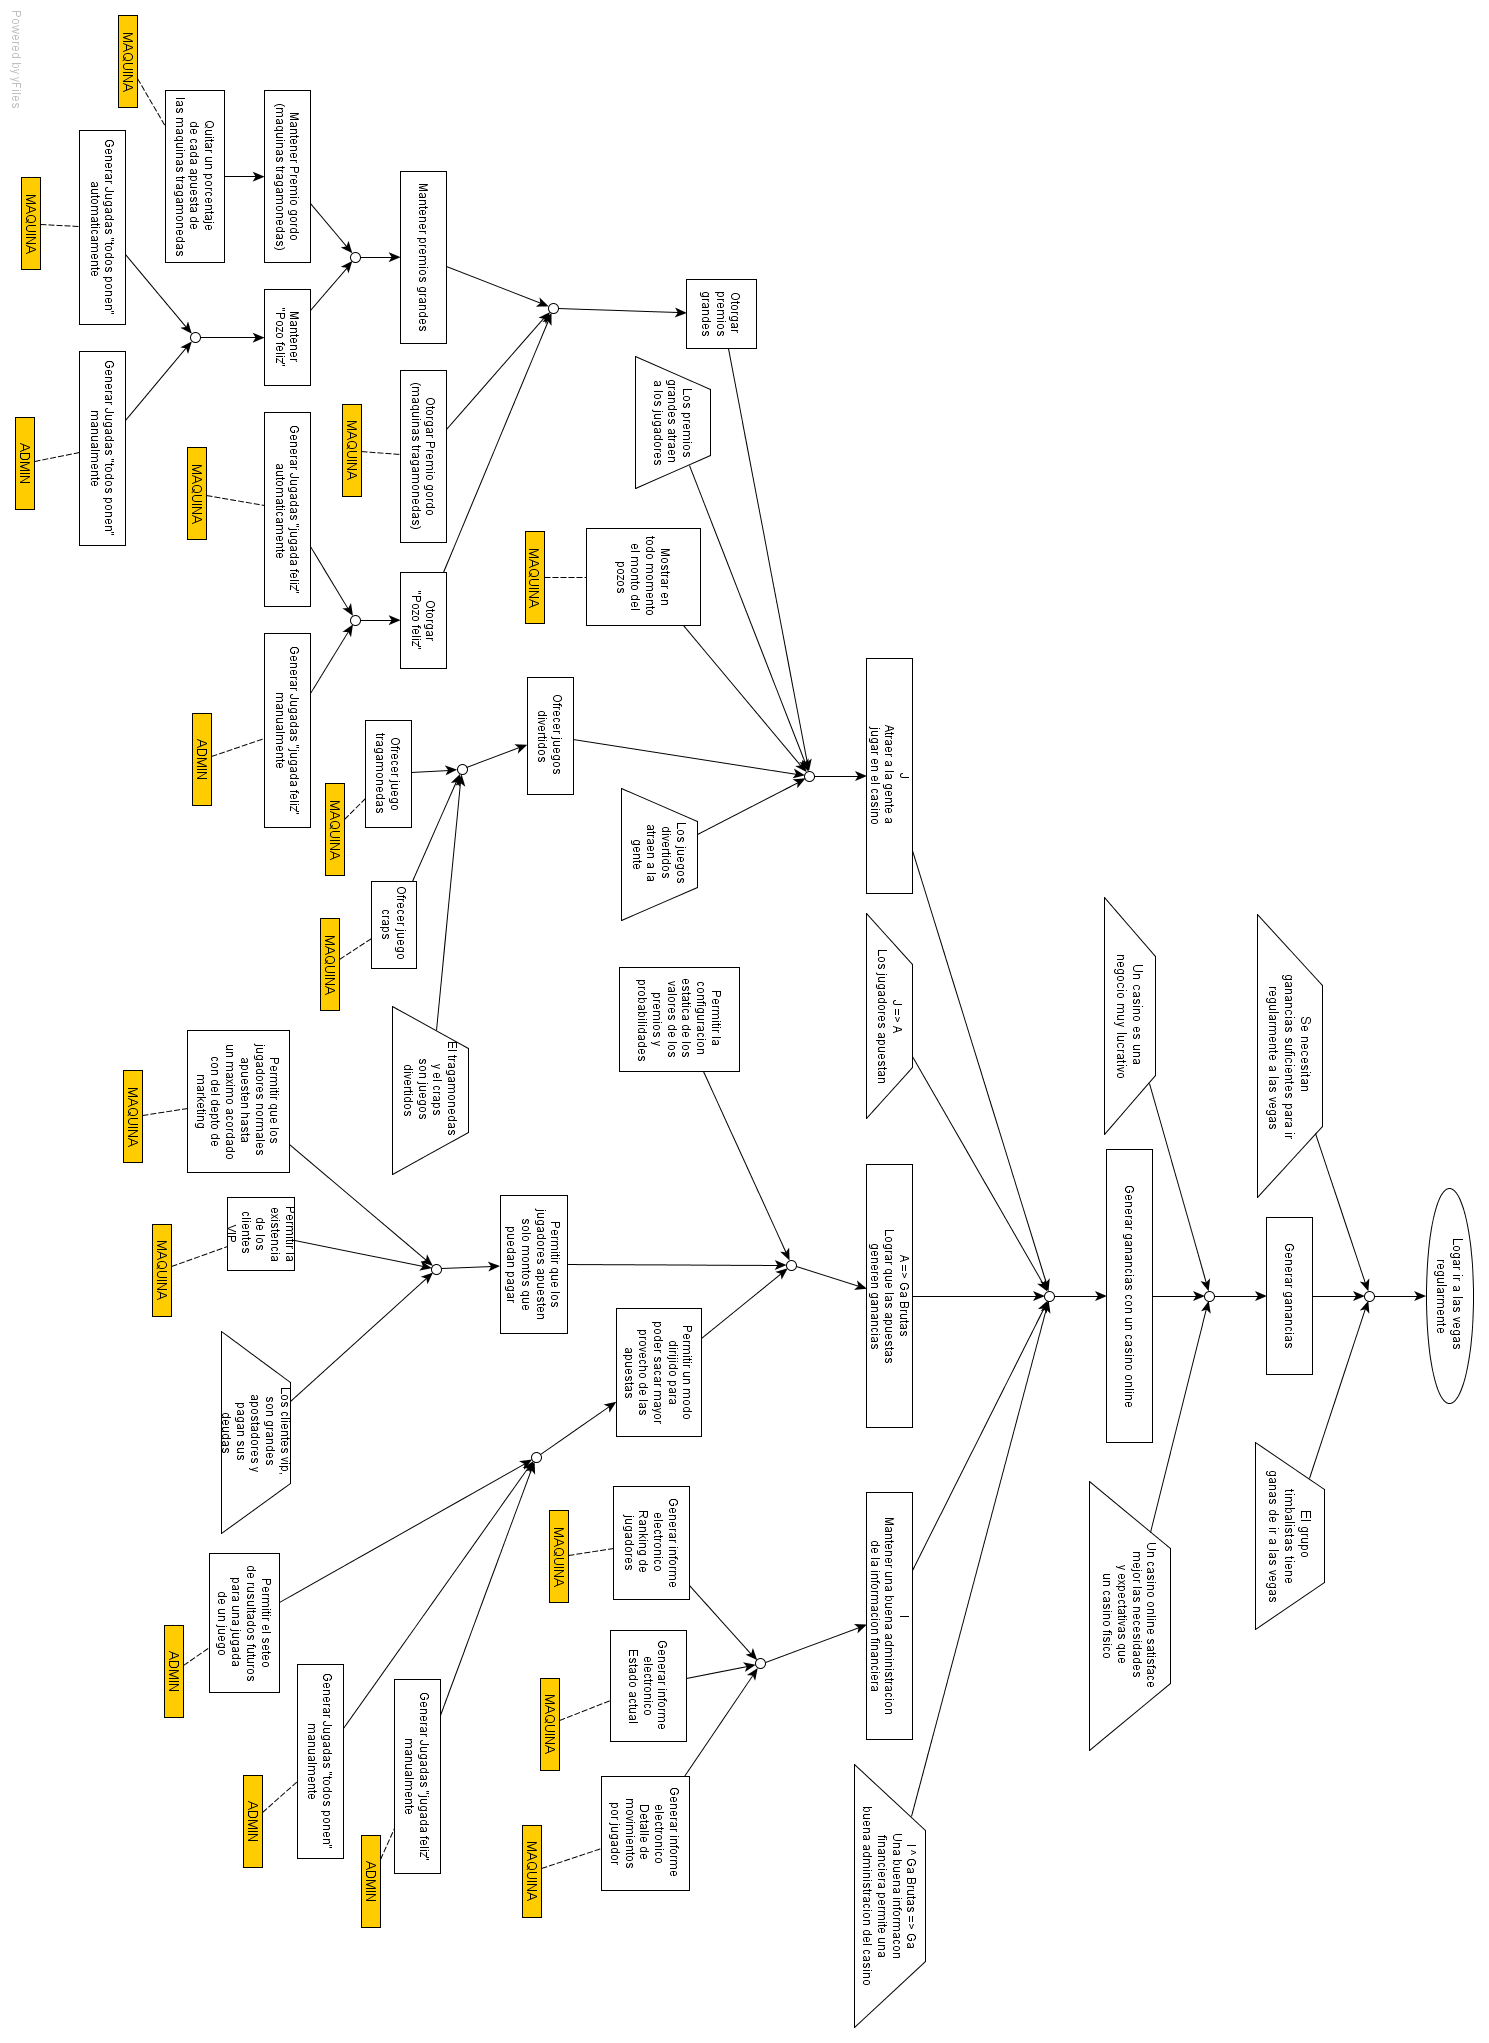
\includegraphics[scale=0.25]{img/doCasino.png}
	\caption{Diagrama de Objetivos \label{fig:doCasino}}
\end{figure}

\begin{framed}

\depto Con este Diagrama de Objetivos intentamos dar el primer paso en la definicion del alcance del sistema y la justificacion de los requerimientos encontrados.
Tambien sera de utilidad para el analisis de los supuestos sobre los que se basar� el sistema.

\end{framed}

\subsection{Analisis de agentes involucrados}

Para comprender mejor la manera en que deberan relacionarse los distintos sujetos del mundo con el sistema a construir y sus interacciones, estucturamos el mundo con un Diagrama de contexto\footnote{Diagrama de contexto: Diagrama donde las cajas son agentes activos del sistema y las flechas son las interacciones basicas}

Este diagrama tambien nos da otra mirada del alcance y expectativas del software a construir.

\begin{figure}[h!]
	\centering
		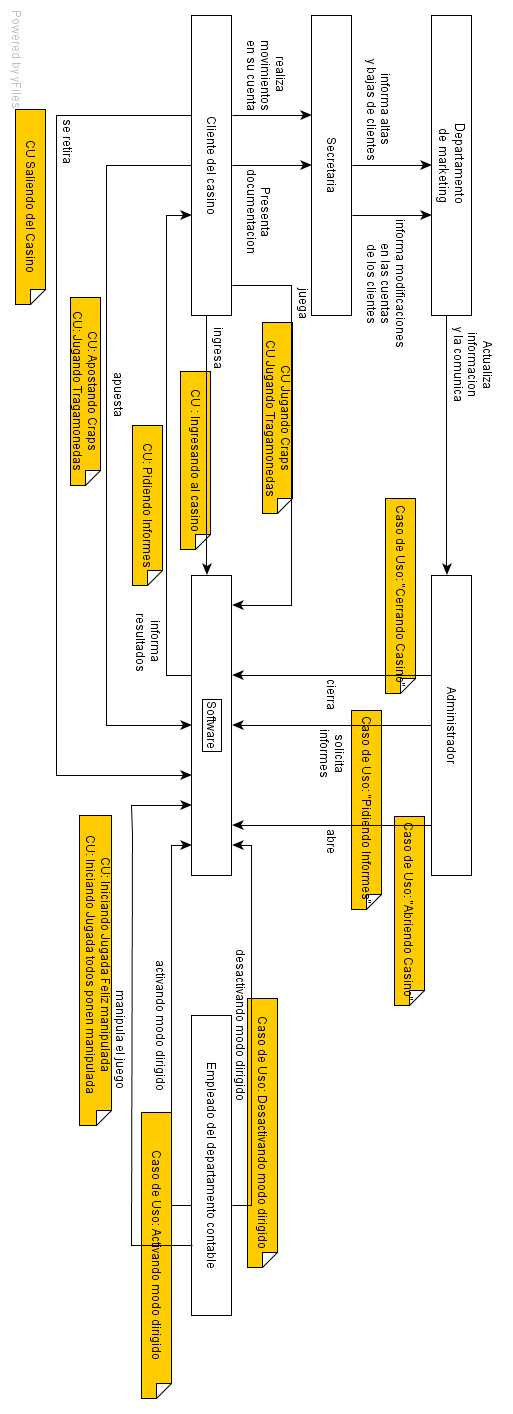
\includegraphics[scale=0.38]{img/dcCasino.png}
	\caption{Diagrama de Contexto \label{fig:dcCasino}}
\end{figure}

\begin{framed}

\depto Todas las interacciones de los agentes con el sistema han sido asignadas a uno o mas Casos de Uso que explicaran de forma mas detallada dichas interacciones. De esta manera podemos garantizar que las interacciones mas relevantes del sistema seran correctamente detalladas

\end{framed}

\subsection{Lista de Requerimientos}

\newcommand{\ii}{{\bf Importante }}
\newcommand{\ff}{{\bf Funcional }}
\newcommand{\dd}{{\bf Deseable }}
\newcommand{\nd}{{\bf No deseable }}
\newcommand{\nf}{{\bf No funcional }}
\newcommand{\ee}{{\bf Esencial }}

\newcommand{\rrr}{{ \\ \bf REFERIDO EN: }}

\begin{enumerate}

\item\textsc{REQUERIMIENTOS GENERALES DEL CASINO - MANEJO DE CLIENTES}
\begin{enumerate}
\item Los clientes no podr�n apostar mas que el saldo permitido por el departamento de marketing: Los clientes tendr�n un saldo limite y no podr�n realizar ningun tipo de apuesta que sobrepase ese saldo.  \ff - \ii. \rrr \ref{1a1} y en \ref{1a2}
\item Los clientes VIP podr�n apostar ilimitadamente: Los clientes VIP no tiene limite de saldo, por lo tanto no habra ningun monto de apuesta que pueda ser invalidado.  \ff - \ii. \rrr \ref{1b1} y en \ref{1b2}
\item VER Un invitado podr� observar los juegos pero sin participar en ellos: Puede ingresar en una mesa ya abierta y observar el desarrollo del juego pero sin intervenir en el. \ff - \dd. \rrr \ref{1c}
\item Se deber� modificar el saldo del cliente en cada apuesta: Cada vez que un cliente haga una apuesta de cualquier tipo se vera reflejado en la disminuci�n de su saldo.  \ff - \ii. \rrr \ref{1d1} y en \ref{1d2}
\end{enumerate}

\item\textsc{REQUERIMIENTOS GENERALES DEL CASINO - MANEJO DE MESAS}
\begin{enumerate}
\item No se debe permitir que un jugador juegue en mas de una mesa al mismo tiempo: Para ingresar a una mesa de cualquier juego el jugador no podr� estar adentro de ninguna otra mesa de ningun juego.  \ff - \dd. \rrr \ref{2a1} y en \ref{2a2}
\item Los clientes podr�n abrir mesas: Todos los clientes tendran la opci�n de abrir una nueva mesa para cualquiera de los juegos.  \ff - \ee
\item Los clientes podr�n unirse a mesas (s� el juego lo permite): El tragamonedas no permite unirse a una mesa, pero en el Craps el jugador podr� elegir a cual de las mesas habilitadas se unir�.  \ff - \ii
\item Las mesas vacias se cerraran autom�ticamente: Cuando un jugador salga de un juego el sitema autom�ticamente cerrara la mesa a menos que haya otros jugadores en ella.  \ff - \ee
\item El casino no se podr� cerrar mientras haya gente jugando: El casino solo podr� cerrar cuando todos los jugadores hayan salido del mismo.  \ff - \ii
\item No debe haber limite de mesas abiertas: Los clientes podr�n ingresar a las mesas de los juegos y no habra un limite de ellas.  \ff - \ii
\end{enumerate}

\item\textsc{REQUERIMIENTOS GENERALES DEL CASINO - PANTALLA}
\begin{enumerate}
\item Las pantallas mostraran la informaci�n necesaria para el desarrollo del juego: Las pantallas mostrar�n la interfaz del juego asi como tambien todas las opciones disponibles dentro del juego.  \ff - \ii
\item Las pantallas mostraran la informaci�n necesaria del estado del juego: Las pantallas mostraran el tipo de jugada, estado actual del juego y resultados, y ser� inmediatamente actualizada ante cualquier cambio o variaci�n.  \ff - \ii
\item Las pantallas mostraran el estado de la cuenta del jugador: Por pantalla se podr� ver si un jugador esta dentro del casino y dentro de algun juego y si es as� en que mesa, si ha resultado ganador o no, y su correspondiente saldo.  \ff - \dd
\end{enumerate}

\item\textsc{REQUERIMIENTOS GENERALES DEL CASINO - CONFIGURACION}
\begin{enumerate}
\item Permitir la configuraci�n est�tica del monto m�nimo de los pozos: Se podr� permitir configurar el monto minimo que debe superar un pozo antes de poder entregarlo.  \nf - \dd
\end{enumerate}

\item\textsc{REQUERIMIENTOS GENERALES DEL CASINO - FICHAS}
\begin{enumerate}
\item Las apuestas se har�n por medio de fichas: En todos los juegos el jugador podr� elegir el monto a apostar seleccionando de entre los valores establecidos de las fichas.  \ff - \ii
\item Las fichas ser�n ilimitadas: No habra una cantidad fija de fichas sino que se dispondr� de ellas en un numero ilimitado.  \ff - \ii
\item El valor de las fichas debe poder configurarse por el administrador: Cada vez que el casino abre al administrador configurara los valores posibles de las fichas.  \nf - \ii
\end{enumerate}

\item\textsc{REQUERIMIENTOS GENERALES DEL CASINO - REPORTES}
\begin{enumerate}
\item Generar informe electr�nico: Ranking de jugadores: Se generar� un informe con los jugadores que m�s dinero ganaron en el d�a desde que abrio el casino, como tambi�n los que m�s dinero perdieron. \ff - \ii
\item Generar informe electronico: Estado Actual: Se generar� un informe con el estado del casino y su saldo y tambi�n el de los clientes. \ff - \ii
\item Generar informe electronico: Detalle de movimientos por jugador: Se generar� un informe con todas las apuestas, premios ganados, y montos ganados por cada jugador que haya ingresado al casino. \ff - \ii
\end{enumerate}

\item\textsc{REQUERIMIENTOS GENERALES DEL CASINO - JUGADAS Y POZOS}
\begin{enumerate}
\item Mostrar en todo momento el monto de los pozos: En todo momento se mostrara el monto actualizado de todos los pozos del casino, y se actualizar� inmediatamente a medida que varie. \ff - \ii
\item Generar jugada feliz autom�ticamente: La jugada feliz se generara en base a probabilidades.  \ff - \ee
\item Generar jugada todos ponen autom�ticamente: La jugada todos ponen tambien se generara en base a probabilidades.  \ff - \ee
\item No se debe permitir el solapamiento de jugadas felices en el mismo instante: Si ha ocurrido una, entonces no podra ocurrir otra hasta que se pague la jugada existente y se supere el monto minimo, aunque pueden ocurrir en cualquiera de las mesas del casino pero no simultaneamente.  \ff - \ii
\end{enumerate}

\item\textsc{REQUERIMIENTOS GENERALES DEL CASINO - MODO DIRIGIDO}
\begin{enumerate}
\item El sistema deber� contar con un modo dirigido: Se podra poner en modo dirigido a cada uno de los juegos y todas sus respectivas mesas tendr�n como resultado el definido por el manipulador de modos.  \ff - \ii
\item El sistema deber� permitir generar jugada feliz manualmente: El manipulador de modos podr� decidir la ocurrencia de jugadas felices mientras no se solapen simultaneamente en los juegos del casino.  \ff - \ii
\item El sistema deber� permitir generar jugada todos ponen manualmente: El manipulador de modos podr� decidir la ocurrencia de jugadas todos ponen mientras no se solapen en la misma jugada. \ff - \ii
\end{enumerate}

\item\textsc{REQUERIMIENTOS DE JUEGO TRAGAMONEDAS}
\begin{enumerate}
\item Proveer juego Tragamonedas: Se proveera el juego del Tragamonedas respetando las reglas provistas por los clientes.  \ff - \ee. \rrr \ref{9a}
\item El juego Tragamonedas debe contar con un premio gordo progresivo: El juego de Tragamonedas permitira incrementar el premio gordo progresivo usando un porcentaje de cada una de las jugadas para ser otorgado luego de superar el monto minimo configurado al que obtenga la combinacion ganadora y haya apostado las n veces anteriores al maximo numero de fichas. \ff - \ee. \rrr \ref{9b}
\item El cliente podr� elegir entre varios valores de fichas de las maquinas tragamonedas: Se podr� elegir una mesa de maquina tragamonedas de distintos valores entre los definidos. Una vez elegido el valor de la ficha para el tragamonedas este no se podr� cambiar hasta salir del juego.  \ff - \nd. \rrr \ref{9c}
\end{enumerate}

\item\textsc{REQUERIMIENTOS DE JUEGO CRAPS}
\begin{enumerate}
\item Proveer juego Craps: Se proveera el juego de Craps respetando las reglas provistas por los clientes. \ff - \ee. \rrr \ref{10a}
\end{enumerate}

\item\textsc{REQUERIMIENTOS DE IMPLEMENTACION Y COMPORTAMIENTO}
\begin{enumerate}
\item El sistema debe funcionar en red.  \nf - \ee
\item VER El sistema a implementarse deber� estar realizado en Java o C$\#$ \nf - \ii 
\item VER El sistema debe ser facilmente extendible con nuevos juegos \nf - \ii 
\end{enumerate}


\item\textsc{REQUERIMIENTOS DE FUNCIONALIDAD EXTRA}
\begin{enumerate}
\item VER Se podr�n ver imagenes de los juegos en 3D \ff - \dd
\item VER Los jugadores podran chatear entre ellos dentro del juego \ff - \dd
\end{enumerate}

\end{enumerate}




\begin{framed}
\textbf{TINTERO: } Nos ha quedado en el tintero relacionar en el imforme los requerimientos con las distintas secciones del trabajo.\\
De todas maneras utilizamos esta lista de el modelo de objetivos como base para evaluar completitud de este informe.\\
Tambien hemos realizado otros tipos de trazabilidad con otros modelos.
\end{framed}

\newpage
\subsection{Modelo Conceptual}

Identificamos y explicamos los conceptos funadamentales y las propiedades definitorias de ellos, y los estructuramos en un Modelo Conceptual\footnote{Casa caja representa una agrupacion de objetos reconocidos del dominio del problema que se caracterizan por tener propiedades similares, las lineas son asociaciones estre estos conceptos que indica alguna vinculacion significativa entre ellos}

\begin{center}
		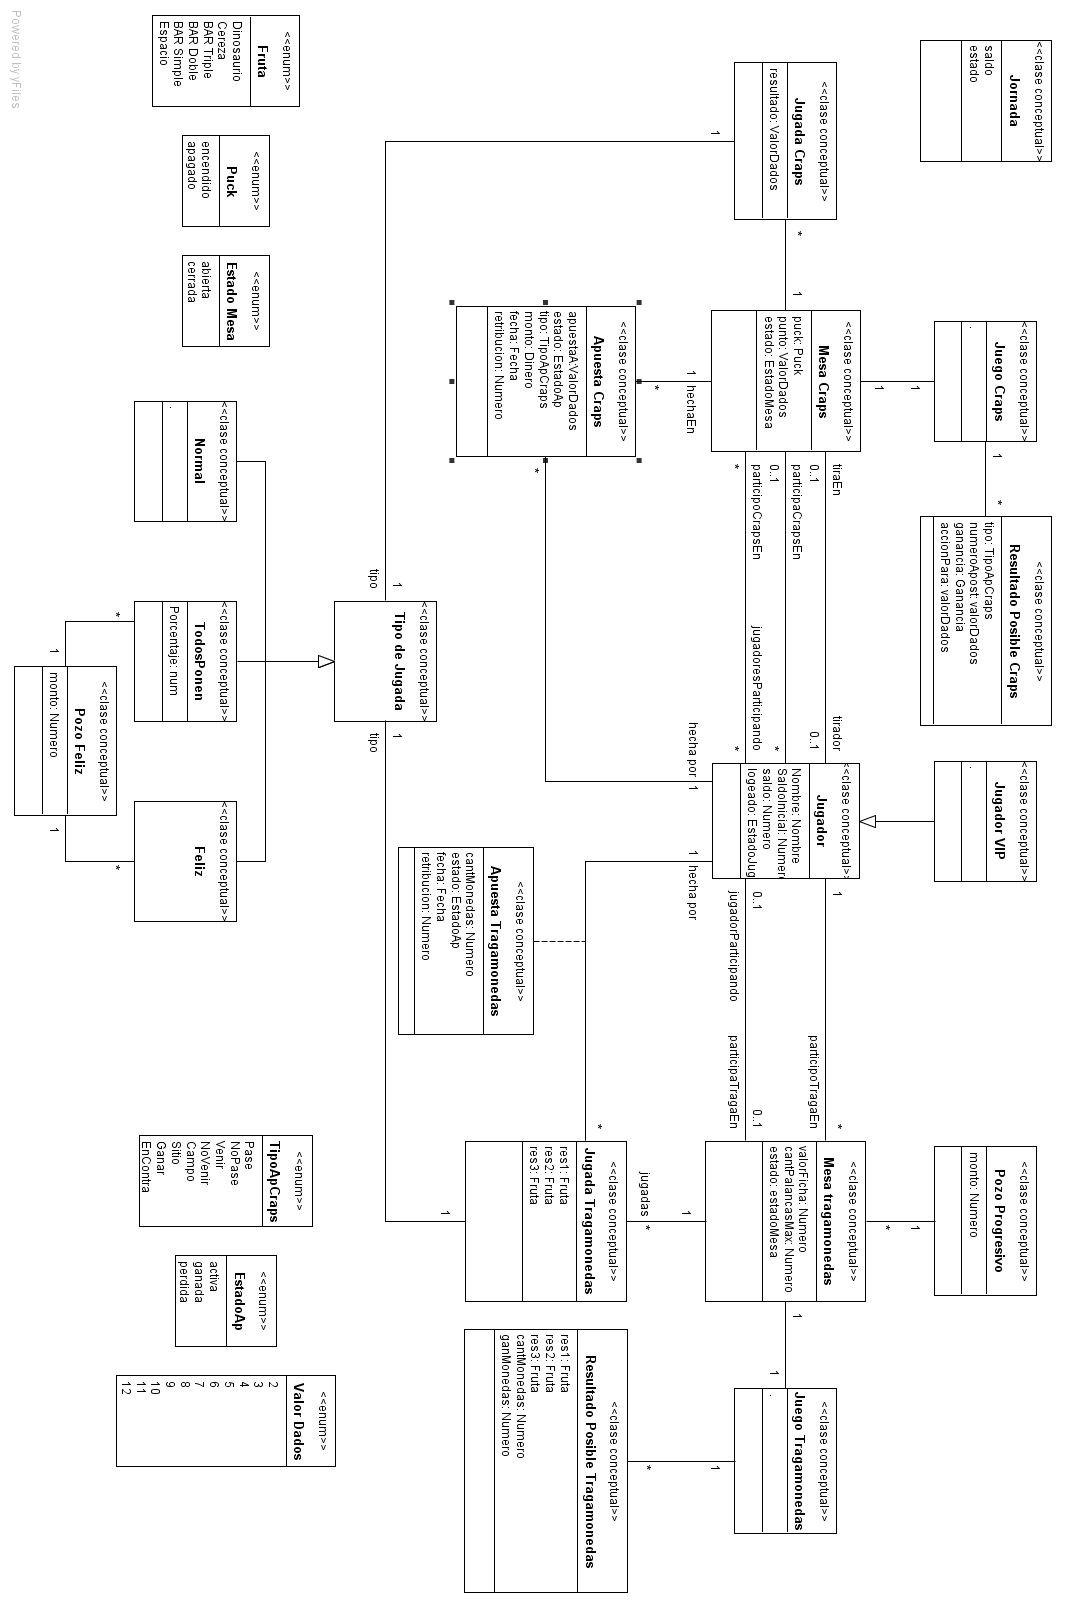
\includegraphics[scale=0.38]{img/dclCasino.png}
\end{center}

Dado las limitaciones del Modelo Conceptual, agregaremos algunos invarientes para identificar mejor los estados deseables del sistema. Ver Anexo \ref{an2}


\subsection{Casos de Uso}

\begin{figure}[h!]
	\centering
		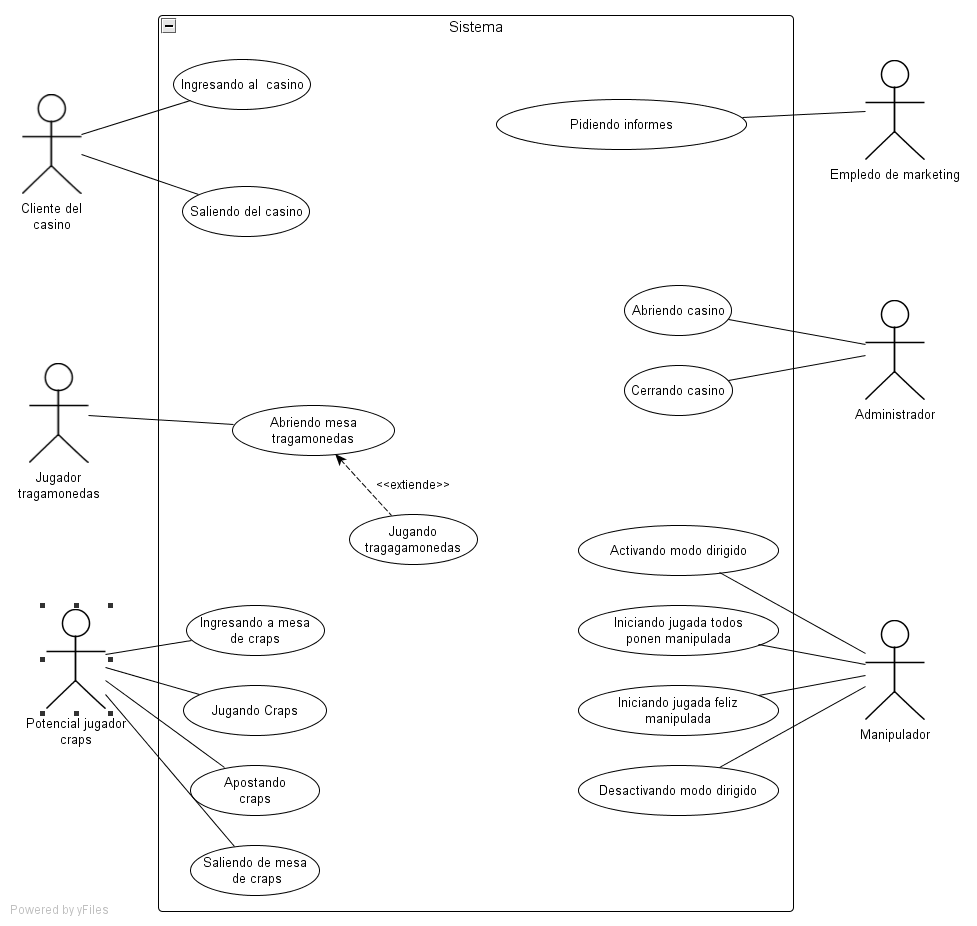
\includegraphics[scale=0.38]{img/casosDeUso.png}
	\caption{Casos de Uso \label{fig:cuCasino}}
\end{figure}

\begin{figure}[h!]
	\centering
		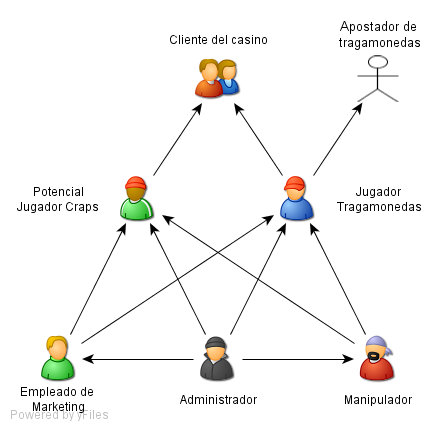
\includegraphics[scale=0.38]{img/herencia.png}
	\caption{Casos de Uso \label{fig:herencia}}
\end{figure}

%%%%%%%ACTORES
%%%%%%\newcommand{\pc}{{\bf Cliente del casino }}
%%%%%%\newcommand{\adm}{{\bf Administrador }}
%%%%%%%\newcommand{\ptra}{{\bf Potencial jugador de tragamonedas }}
%%%%%%\newcommand{\jutra}{{\bf Jugador de Tragamonedas }}
%%%%%%\newcommand{\jc}{{\bf Jugador de Craps }}
%%%%%%\newcommand{\jac}{{\bf Apostador de Craps }}
%%%%%%\newcommand{\emc}{{\bf Empleado Contable }}
%%%%%%\newcommand{\emk}{{\bf Empleado de Marketing }}
%%%%%%\newcommand{\aptra}{{\bf Apostador de Tragamonedas }}
%%%%%%\newcommand{\apocr}{{\bf Apostador de Craps }}
%%%%%%\newcommand{\jucr}{{\bf Potencial Jugador de Craps }}
%%%%%%%CASOS DE USO
%%%%%%\newcommand{\ic}{{\bf Ingresando a casino }}
%%%%%%\newcommand{\salc}{{\bf Saliendo del casino }}
%%%%%%\newcommand{\atra}{{\bf Abriendo Mesa Tragamonedas }}
%%%%%%\newcommand{\jtra}{{\bf Jugando Tragamonedas }}
%%%%%%\newcommand{\actm}{{\bf Activando Modo Dirigido }}
%%%%%%\newcommand{\desm}{{\bf Desactivando Modo Dirigido }}
%%%%%%\newcommand{\jugf}{{\bf Jugada Feliz }}
%%%%%%\newcommand{\jugtp}{{\bf Jugada Todos Ponen }}
%%%%%%\newcommand{\ac}{{\bf Abriendo Casino }}
%%%%%%\newcommand{\cc}{{\bf Cerando Casino }}
%%%%%%\newcommand{\apotra}{{\bf Apostando en Tragamonedas }}
%%%%%%\newcommand{\incr}{{\bf Ingresando a mesa de Craps }}
%%%%%%\newcommand{\scr}{{\bf Saliendo de mesa de Craps }}
%%%%%%\newcommand{\jcr}{{\bf Jugando Craps }}
%%%%%%\newcommand{\apcr}{{\bf Apostando Craps }}
%%%%%%\newcommand{\admin}{{\bf administrador}}
%%%%%%\newcommand{\ccas}{{\bf Cerrando Casino}}
%%%%%%\newcommand{\empmark}{{\bf Empleado de Marketing}}
%%%%%%\newcommand{\infomovjug}{{\bf Pidiendo informes}}
%%%%%%\newcommand{\infoestact}{{\bf informe Estado Actual}}
%%%%%%\newcommand{\inforankjug}{{\bf informe Ranking de Jugadores}}
%%%%%%\newcommand{\infdmj}{{\bf Pidiendo informe Detalles de movimientos por jugador}}
%%%%%%\newcommand{\infea}{{\bf Pidiendo informe Estado Actual}}
%%%%%%\newcommand{\infrj}{{\bf Pidiendo informe Ranking de Jugadores}}


\newcommand{\req}{{\bf Requerimientos satisfechos por este Caso de Uso: }}
%ACTORES
\newcommand{\pc}{{\bf Cliente del casino }}
\newcommand{\adm}{{\bf Administrador }}
\newcommand{\invi}{{\bf Invitado }}
%\newcommand{\ptra}{{\bf Potencial jugador de tragamonedas }}
\newcommand{\jutra}{{\bf Jugador de Tragamonedas }}
\newcommand{\pjc}{{\bf Potencial jugador de Craps }}
\newcommand{\jc}{{\bf Jugador de Craps }}
\newcommand{\apcr}{{\bf Apostador de Craps }}
\newcommand{\emc}{{\bf Empleado Contable }}
\newcommand{\emk}{{\bf Empleado de Marketing }}
\newcommand{\jucr}{{\bf Tirador de Craps}}
\newcommand{\mani}{{\bf Manipulador }}
%CASOS DE USO
\newcommand{\ic}{{\bf Ingresando al casino }}
\newcommand{\salc}{{\bf Saliendo del casino }}
\newcommand{\inginvi}{{\bf Ingresando al casino como invitado}}
\newcommand{\salinvi}{{\bf Saliendo del casino como invitado }}
\newcommand{\obser}{{\bf Observando Juego }}
\newcommand{\intr}{{\bf Ingresando a mesa de Tragamonedas }}
\newcommand{\jtra}{{\bf Jugando Tragamonedas }}
\newcommand{\satr}{{\bf Saliendo a mesa de Tragamonedas }}
\newcommand{\incr}{{\bf Ingresando a mesa de Craps }}
\newcommand{\jugcr}{{\bf Jugando Craps }}
\newcommand{\apocr}{{\bf Apostando Craps }}
\newcommand{\sacr}{{\bf Saliendo a mesa de Craps }}
\newcommand{\actm}{{\bf Activando Modo Dirigido }}
\newcommand{\desm}{{\bf Desactivando Modo Dirigido }}
\newcommand{\jugf}{{\bf Iniciando Jugada Feliz Manipulada}}
\newcommand{\jugtp}{{\bf Iniciando Jugada Todos Ponen Manipulada}}
\newcommand{\ac}{{\bf Abriendo Casino }}
\newcommand{\cc}{{\bf Cerrando Casino }}
\newcommand{\infdmj}{{\bf Pidiendo informe Detalles de movimientos por jugador}}
\newcommand{\infea}{{\bf Pidiendo informe Estado Actual}}
\newcommand{\infrj}{{\bf Pidiendo informe Ranking de Jugadores}}

